\documentclass[11pt]{beamer}
\usepackage{graphicx}
\usepackage{multicol}
\usepackage{tabularx}
\usepackage[toc]{appendix}
\usepackage{amssymb}
\usepackage{amsmath}
\usepackage{datetime}
\usepackage{amsthm}
\usepackage{tikz}
\usetikzlibrary{arrows.meta}
\usetikzlibrary{shapes.multipart}
\usetikzlibrary{patterns}
\usepackage{algorithm}
\usepackage{algpseudocode}
\usepackage{pdfpages}
\usepackage{hyperref}
\usepackage{framed}

\theoremstyle{definition}
\newtheorem{definition}{Definition}

\newtheorem{theorem}{Theorem}
\newtheorem{lemma}{Lemma}
\newtheorem{proposition}{Proposition}
\newtheorem{corollary}{Corollary}

\setlength{\parindent}{0pt}

\newcommand{\reporttitle}{Explaining Makespan Scheduling}
\newcommand{\reportauthor}{Myles Lee}
\newcommand{\supervisor}{Dr. Kristijonas \v{C}yras\\Dr. Dimitrios Letsios}
\newcommand{\marker}{Dr. Ruth Misener}
\newcommand{\reporttype}{MEng. Individual Project}
\newcommand{\toolname}{Schedule Explainer}
\newcommand{\linespace}{\vspace*{\baselineskip}\\}
\newcommand{\pair}[2]{\langle{#1},{#2}\rangle}
\newcommand{\triple}[3]{\langle{#1},{#2},{#3}\rangle}
\newcommand{\intset}[1]{[\![{#1}]\!]}

\tikzstyle{file} = [draw, inner sep=10pt]
\tikzstyle{node} = [draw, circle, minimum size=0.75cm]
\tikzstyle{arrow} = [-{Stealth[scale=2]}]
\tikzstyle{shaded} = [fill=black!15]
\tikzstyle{dot} = [inner sep=2pt,outer sep=0pt, circle, fill=black]

\makeatletter
\newcommand{\incircbin}{\mathpalette\@incircbin}
\newcommand\@incircbin[2]{\mathbin{\ooalign{\hidewidth$#1#2$\hidewidth\crcr$#1\bigcirc$}}}

\newenvironment{level}%
{\addtolength{\itemindent}{2em}}%
{\addtolength{\itemindent}{-2em}}

\newcommand{\unchapter}[1]{%
  \begingroup
  \let\@makechapterhead\@gobble % make \@makechapterhead do nothing
  \chapter{#1}
  \endgroup
}

\begin{document}
	\author{Myles Lee}
	\title{Explaining Makespan Schedules}
	\date{25\textsuperscript{th} June 2019}
	
	\begin{frame}[plain]
		\maketitle
	\end{frame}
	
	\begin{frame}
		\frametitle{Introduction}
		\makebox[\textwidth][c]{
			\begin{tikzpicture}
				\node (left) at (0, 0){\includegraphics[scale=0.25]{figures/inefficient_makespan.png}};
				\node (right) at (6, 0){\includegraphics[scale=0.25]{figures/efficient_makespan.png}};
				\draw[thick,->] (left) -- (right) node[midway, above] {optimise};
			\end{tikzpicture}
		}
		\begin{itemize}
			\item Solvers and schedules are difficult to understand
			\item Apply argumentation to makespan schedules to generate explanations
		\end{itemize}
	\end{frame}

	\begin{frame}
		\frametitle{Contributions}
		\begin{columns}
			\begin{column}{0.5\textwidth}
				\includegraphics[width=\textwidth]{figures/tool_gui.png}
			\end{column}
			\begin{column}{0.5\textwidth}
				\resizebox{\textwidth}{!}{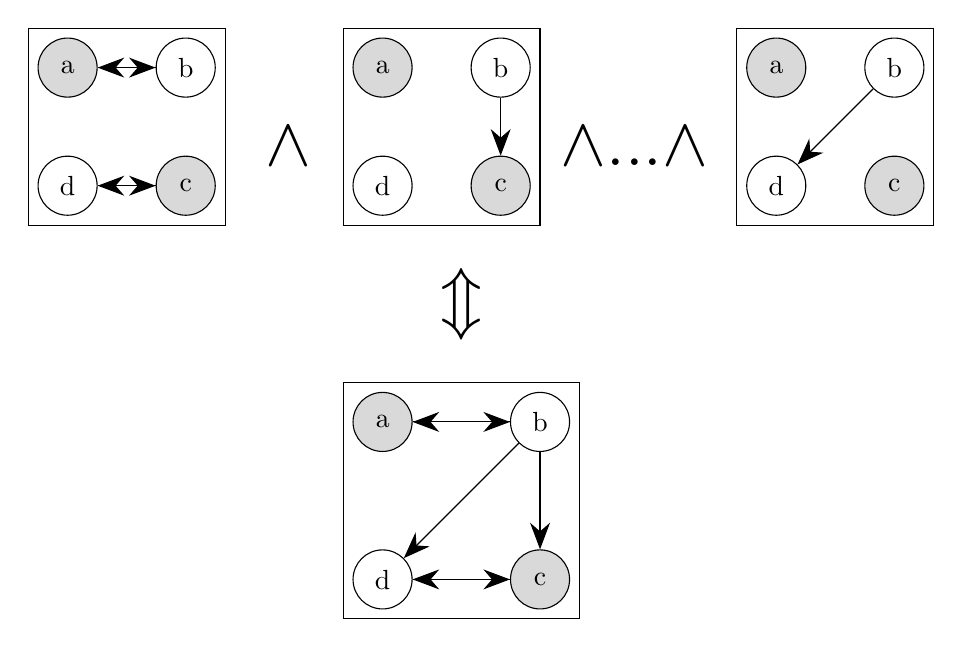
\begin{tikzpicture}
	\node[node, shaded](a) at (0, 1.5){a};
	\node[node](b) at (1.5, 1.5){b};
	\node[node, shaded](c) at (1.5, 0){c};
	\node[node](d) at (0, 0){d};
	\draw[arrow](a) -- (b);
	\draw[arrow](b) -- (a);
	\draw[arrow](c) -- (d);
	\draw[arrow](d) -- (c);
	\draw(-0.5,-0.5) rectangle (2,2);
	\node at (2.8, 0.5){\Huge{$\land$}};

	\node[node, shaded](a) at (4, 1.5){a};
	\node[node](b) at (5.5, 1.5){b};
	\node[node, shaded](c) at (5.5, 0){c};
	\node[node](d) at (4, 0){d};
	\draw[arrow](b) -- (c);
	\draw(3.5,-0.5) rectangle (6,2);
	\node at (7.2, 0.5){\Huge{$\land...\land$}};

	\node[node, shaded](a) at (9, 1.5){a};
	\node[node](b) at (10.5, 1.5){b};
	\node[node, shaded](c) at (10.5, 0){c};
	\node[node](d) at (9, 0){d};
	\draw[arrow](b) -- (d);
	\draw(8.5,-0.5) rectangle (11,2);
	\node at (5, -1.5){\Huge{$\Updownarrow$}};

	\node[node, shaded](a) at (4, -3){a};
	\node[node](b) at (6, -3){b};
	\node[node, shaded](c) at (6, -5){c};
	\node[node](d) at (4, -5){d};
	\draw[arrow](a) -- (b);
	\draw[arrow](b) -- (a);
	\draw[arrow](b) -- (c);
	\draw[arrow](b) -- (d);
	\draw[arrow](c) -- (d);
	\draw[arrow](d) -- (c);
	\draw(3.5,-5.5) rectangle (6.5, -2.5);
\end{tikzpicture}}
			\end{column}
		\end{columns}

		\begin{columns}
			\begin{column}{0.5\textwidth}
				\begin{itemize}
					\item Interactive tool
					\item Algorithms
				\end{itemize}
			\end{column}
			\begin{column}{0.5\textwidth}
				\begin{itemize}
					\item Theoretical extensions 
					\item Discussion
				\end{itemize}
			\end{column}
		\end{columns}			
	\end{frame}

	\begin{frame}
		\frametitle{Demonstration}
		\includegraphics[width=\textwidth]{figures/tool_gui.png}
	\end{frame}

	\begin{frame}
		\frametitle{Pipeline}
		\resizebox{\textwidth}{!}{\begin{tikzpicture}
	\node[draw, align=center] (problem) at (0, 3){$m=2$\\$n=3$\\$\mathbf{p}=[2,4,5]$\\$D=\varnothing$};

	\draw(2,2) rectangle (4, 4);
	\node[draw, circle] (a) at (2.5, 2.5){};
	\node[draw, circle] (b) at (3, 2.5){};
	\node[draw, circle] (c) at (3.5, 2.5){};
	\node[draw, circle] (d) at (2.5, 3.5){};
	\node[draw, circle] (e) at (3, 3.5){};
	\node[draw, circle] (f) at (3.5, 3.5){};
	\draw[<->] (a) -- (d);
	\draw[<->] (b) -- (e);
	\draw[<->] (c) -- (f);

	\node (chart) at (0, 0){\includegraphics[scale=0.15]{figures/tiny_makespan.png}};
	\node (matrix) at (3, 0){$\begin{bmatrix}
		1 & 0 & 1\\
		0 & 1 & 0\\
		\end{bmatrix}$
	};

	\draw(5,0) rectangle (7, 2);
	\node[draw, circle] (a) at (5.5, 0.5){};
	\node[shaded,draw, circle] (b) at (6, 0.5){};
	\node[draw, circle] (c) at (6.5, 0.5){};
	\node[shaded,draw, circle] (d) at (5.5, 1.5){};
	\node[draw, circle] (e) at (6, 1.5){};
	\node[shaded,draw, circle] (f) at (6.5, 1.5){};
	\draw[<->] (a) -- (d);
	\draw[<->] (b) -- (e);
	\draw[<->] (c) -- (f);
	
	\node[draw](text) at (9, 1){Explanation};
	
	\draw[arrow] (problem) -- (2, 3);
	\draw[arrow, dashed] (problem) -- (chart);
	\draw[arrow] (4, 2.333) -- (5, 1.666);
	\draw[arrow] (chart) -- (matrix);
	\draw[arrow] (matrix) -- (5, 0.666);
	\draw[arrow] (7, 1) -- (text);
\end{tikzpicture}}
	\end{frame}

	\begin{frame}
		\frametitle{Abstract Argumentation}
		\begin{itemize}
			\item An abstract argumentation framework is a directed graph $\pair{Args}{\rightsquigarrow}$.
			\item Extension $E$ is a subset of $Args$.
		\end{itemize}
		
		\begin{definition}
			$E$ is conflict-free on $\pair{Args}{\rightsquigarrow}$ iff $\forall a,b\in E. a\not\rightsquigarrow b$.
		\end{definition}
	
		\begin{definition}
			$E$ is stable on $\pair{Args}{\rightsquigarrow}$ iff $E$ is conflict-free on $\pair{Args}{\rightsquigarrow}$ and $\forall a\in Args\setminus E.\exists e\in E.e\rightsquigarrow a$.
		\end{definition}
	\end{frame}

	\begin{frame}
		\frametitle{Theorem}
		\begin{center}
			\resizebox{0.9\textwidth}{!}{\input{theorem}}		
		\end{center}
	\end{frame}
\end{document}